\documentclass[a4paper,12pt]{article}
%%% Работа с русским языком
\usepackage[unicode, pdftex]{hyperref}
\usepackage{cmap}					% поиск в PDF
\usepackage{mathtext} 				% русские буквы в формулах
\usepackage[T2A]{fontenc}			% кодировка
\usepackage[utf8]{inputenc}			% кодировка исходного текста
\usepackage[english,russian]{babel}	% локализация и переносы
\usepackage{indentfirst}
\frenchspacing


\renewcommand{\epsilon}{\ensuremath{\varepsilon}}
\renewcommand{\phi}{\ensuremath{\varphi}}
\renewcommand{\kappa}{\ensuremath{\varkappa}}
\renewcommand{\le}{\ensuremath{\leqslant}}
\renewcommand{\leq}{\ensuremath{\leqslant}}
\renewcommand{\ge}{\ensuremath{\geqslant}}
\renewcommand{\geq}{\ensuremath{\geqslant}}
\renewcommand{\emptyset}{\varnothing}

%%% Дополнительная работа с математикой
\usepackage{amsmath,amsfonts,amssymb,amsthm,mathtools} % AMS
\usepackage{icomma} % "Умная" запятая: $0,2$ --- число, $0, 2$ --- перечисление

%% Номера формул
%\mathtoolsset{showonlyrefs=true} % Показывать номера только у тех формул, на которые есть \eqref{} в тексте.
%\usepackage{leqno} % Нумереация формул слева

%% Свои команды
\DeclareMathOperator{\sgn}{\mathop{sgn}}

%% Перенос знаков в формулах (по Львовскому)
\newcommand*{\hm}[1]{#1\nobreak\discretionary{}
	{\hbox{$\mathsurround=0pt #1$}}{}}

%%% Работа с картинками
\usepackage{graphicx}  % Для вставки рисунков
%\graphicspath{{images/}{images2/}}  % папки с картинками
\setlength\fboxsep{3pt} % Отступ рамки \fbox{} от рисунка
\setlength\fboxrule{1pt} % Толщина линий рамки \fbox{}
\usepackage{wrapfig} % Обтекание рисунков текстом

%%% Работа с таблицами
\usepackage{array,tabularx,tabulary,booktabs} % Дополнительная работа с таблицами
\usepackage{longtable}  % Длинные таблицы
\usepackage{multirow} % Слияние строк в таблице

%%% Теоремы
\theoremstyle{plain} % Это стиль по умолчанию, его можно не переопределять.
\newtheorem{theorem}{Теорема}[section]
\newtheorem{proposition}[theorem]{Утверждение}

\theoremstyle{definition} % "Определение"
\newtheorem{corollary}{Следствие}[theorem]
\newtheorem{problem}{Задача}[section]

\theoremstyle{remark} % "Примечание"
\newtheorem*{nonum}{Решение}

%%% Программирование
\usepackage{etoolbox} % логические операторы

%%% Страница
\usepackage{extsizes} % Возможность сделать 14-й шрифт
\usepackage{geometry} % Простой способ задавать поля
\geometry{top=25mm}
\geometry{bottom=35mm}
\geometry{left=25mm}
\geometry{right=20mm}
%
\usepackage{fancyhdr} % Колонтитулы
\pagestyle{fancy}
%\renewcommand{\headrulewidth}{0pt}  % Толщина линейки, отчеркивающей верхний колонтитул
% 	\lfoot{Нижний левый}
% 	\rfoot{Нижний правый}
% 	\chead{Верхний в центре}
% 	\lhead{Верхний левый}
%	\cfoot{Нижний в центре} % По умолчанию здесь номер страницы
\usepackage{lastpage}

\fancyhead[L]{}
\fancyhead[C]{}

\usepackage{setspace} % Интерлиньяж (расстояние между строками)
%\onehalfspacing % Интерлиньяж 1.5
%\doublespacing % Интерлиньяж 2
%\singlespacing % Интерлиньяж 1

\usepackage{lastpage} % Узнать, сколько всего страниц в документе.




\usepackage[usenames,dvipsnames,svgnames,table,rgb]{xcolor}
\hypersetup{				% Гиперссылки
	unicode=true,           % русские буквы в раздела PDF
	pdftitle={Заголовок},   % Заголовок
	pdfauthor={Автор},      % Автор
	pdfsubject={Тема},      % Тема
	pdfcreator={Создатель}, % Создатель
	pdfproducer={Производитель}, % Производитель
	pdfkeywords={keyword1} {key2} {key3}, % Ключевые слова
	colorlinks=true,       	% false: ссылки в рамках; true: цветные ссылки
	linkcolor=red,          % внутренние ссылки
	citecolor=black,        % на библиографию
	filecolor=magenta,      % на файлы
	urlcolor=cyan           % на URL
}


%\usepackage[style=authoryear,maxcitenames=2,backend=biber,sorting=nty]{biblatex}

\usepackage{multicol} % Несколько колонок

\usepackage{tikz} % Работа с графикой
\usepackage{pgfplots}
\usepackage{pgfplotstable}
\usepackage{floatrow}
\DeclareFloatSeparators{mysep}{\hspace{3cm}}
\thisfloatsetup{floatrowsep=mysep}


\begin{document}
\section{Аннотация} 
В данной работе были исследованы автоэмиссионные свойства и механизмы нестабильности автоэмиссионного тока на примере катода, изготовленного из углеродных волокон, а также получена ВАХ лампы с помощью осциллографа 

\section{Теория}
	
\subsection*{Теория автоэмиссии}
\textit{Автоэлектронной эмиссией} называется явление испускания электронов в вакуум с поверхности твердого тела или другой среды под действием очень сильного электрического поля напряженностью $F = 10^{7}-10^{8}$В/см.

Из-за необходимой величины поля для АЭЭ используются тонкие острия с радиусом вершины порядка 0,1-0,01 мкм. С уменьшением радиуса кривизны катода падает необходимое для протекания АЭЭ напряжение.

Основной физический процесс при АЭЭ – туннелирование электронов сквозь потенциальный барьер на поверхности тела, барьер искривляется приложенным полем, таким об- разом, что появляется область пространства вне тела, где электрон обладал бы такой же полной энергией, как в теле. Таким образом, АЭЭ обуславливается волновыми свойствами электронов.
Уравнение, связывающее плотность АЭ тока $j$ и напряженность поля - уравнение Фаулера-Нордгейма:
\begin{equation*}
    j = \frac{e^3}{4\pi^2\hbar}\cdot \frac{E^{1/2}_{f}}{W_{a}\varphi^{1/2}}\cdot E^{2}\cdot exp(-\frac{4\sqrt{2m}\varphi^{3/2}}{3e\hbar E})
\end{equation*}
    
где $\varphi = W_{a}-E_{f}$ – работа выхода, $E_{f}$ - энергия Ферми, $W_{a}$ - уровень вакуума.
Формула составлена для температуры в 0 К, однако при 293К разница, вносимая изменением температуры, пренебрежимо мала. Позже уравнение было изменено Нордгеймом путем введения в него функции Нордгейма, уравнение приняло вид:
\begin{equation*}
    j = A' \cdot \frac{E^{2}}{\varphi}\cdot exp(-B'\cdot \frac{\varphi_{3/2}}{E}),
\end{equation*}
где $A' = \frac{e^3}{16\pi^2\hbar}\cdot exp(0,739 \frac{4\sqrt{2m}e^3}{3e\sqrt{\varphi}})$, $B' = 0,965\cdot \frac{4\sqrt{2m}}{3e\hbar}$.

При построении графика зависимости $ln(\frac{j}{E^{2}})$ от $\frac{1}{E}$, график будет представлять собой
прямую, называемую кривой \textit{Фаулера-Нордгейма}, соответствующие координаты - \textit{координаты Фаулера-Нордгейма}. Наклон графика равен:

\begin{equation*}
    S_{FN} = -0,683\cdot s(\frac{3,79\sqrt{E}}{\varphi})\cdot \varphi^{3/2},
\end{equation*}
где $s(y)=\nu(y)-\frac{y}{2}\cdot\frac{d\nu}{dy}$

\subsection*{Одноэмиттерные системы}

В случае системы с одним эмиттером имеем $I = Sj, E = \beta U$ , где $\beta$ - форм-фактор острия. Тогда имеем следующее уравнение для тока:

\begin{equation*}
    I = S_{э}\cdot \frac{1,537\cdot10^{10}}{t^{2}(y_{0})}\cdot\frac{\beta^2U^2}{\varphi}exp(-0,683\cdot\frac{\varphi^{3/2}}{\beta U}\cdot\nu(y_{0})),
\end{equation*}
где $y_{0} = 3,79\cdot\frac{\sqrt{\beta U}}{\varphi}$

График зависимости $ln(\frac{1}{U^2})$ от $\frac{1}{U^2}$ –прямая Фаулера – Нордгейма для тока и напряжения. Наклон графика в таком случае:
\begin{equation}
    tg\alpha = -0,683\cdot\frac{\varphi^{3/2}}{\beta}\cdot s(\frac{3,79\cdot\sqrt{\beta E}}{\varphi}).
\end{equation}

В рабочем диапазоне токов и напряжений имеем $tg\alpha = -0,683\cdot\frac{\varphi^{3/2}}{\beta}$.

\subsection*{Нестабильность автоэмиссионного тока}
Из-за разрушения поверхности эмиссионных центров при работе и адсорбции - десорбции атомов остаточных газов эмиссионный ток может быть нестабильным. В результате измерения ВАХ получается следующая зависимость:
\begin{equation*}
    ln(\frac{1}{U^{2}}) = \hat{A}-\hat{B}\cdot\frac{1}{U},
\end{equation*}

где $\hat{A}=ln(A\cdot N\cdot \frac{1}{\varphi\cdot ln^2(\frac{R}{R})})$, $\hat{B} = B^{*}\cdot r\cdot ln(\frac{R}{r})\cdot\varphi^{3/2}$

Из зависимости \hat{A} от $ln(\hat{B})$ можно качественно получить причину нестабильности тока. При изменении числа центров меняется только \hat{A}; при изменении работы выхода наблюдается линейная зависимость с коэффициентом 1.5; при изменении размеров центров зависимость линейна в координатах $\hat{A} + 2\cdot ln(\hat{B})$  от $e^{-\frac{\hat{A}}{2}}$.

\section{Экспериментальная установка}
В нашей работе исследуются автоэмиссионные свойства и механизмы нестабильности автоэмиссионного тока на примере катодов, изготовленных из углеродных волокон. Исследуемые автокатоды находятся в отпаянной стеклянной лампе, схема которой представлена на рисунке 1.

\begin{figure}[H]
	\centering
	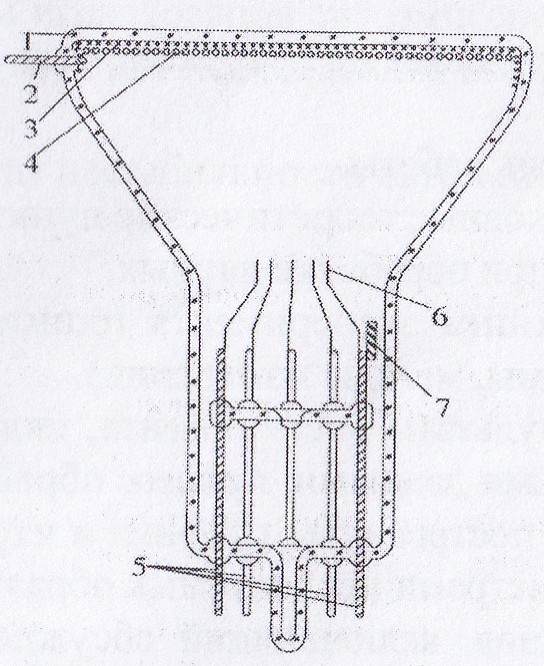
\includegraphics[scale=0.4]{pic1.jpg}
	\caption{Конструкция автоэмиссионной лампы на основе углеродных волокон, для исследования автоэмиссионных свойств углеродных волокон}
	\label{pic2}
\end{figure}

\begin{figure}[H]
	\centering
	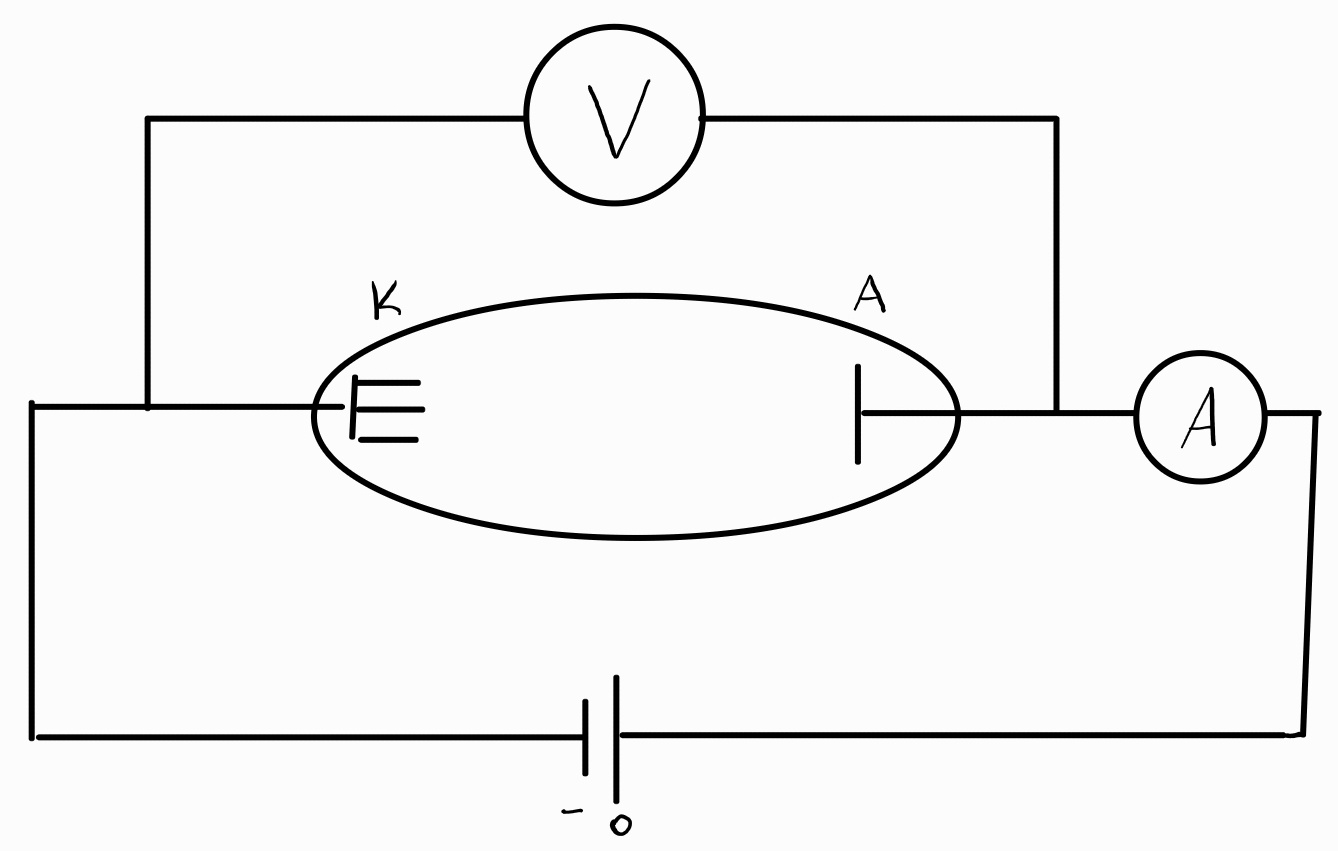
\includegraphics[scale=0.2]{scheme.jpg}
	\caption{Схема экспериментальной установки}
	\label{pic2}
\end{figure}

\section{Ход работы}
 
Снимем ВАХ катода:

\begin{table}[H]
\begin{tabular}{|c|c|}
\hline
I, мА & U, В \\ \hline
0,002 & 1800 \\ \hline
0,01  & 1990 \\ \hline
0,02  & 2064 \\ \hline
0,03  & 2092 \\ \hline
0,045 & 2142 \\ \hline
0,05  & 2206 \\ \hline
0,06  & 2234 \\ \hline
0,07  & 2325 \\ \hline
0,08  & 2388 \\ \hline
0,1   & 2439 \\ \hline
0,11  & 2500 \\ \hline
\end{tabular}
\hspace{1cm}
\begin{tabular}{|c|c|}
\hline
I, мА & U, В \\ \hline
0,12  & 2530 \\ \hline
0,11  & 2458 \\ \hline
0,1   & 2430 \\ \hline
0,08  & 2398 \\ \hline
0,07  & 2357 \\ \hline
0,06  & 2326 \\ \hline
0,05  & 2260 \\ \hline
0,04  & 2200 \\ \hline
0,03  & 2150 \\ \hline
0,02  & 2053 \\ \hline
0,01  & 1930 \\ \hline
\end{tabular}
\caption{ВАХ катода}
\end{table}

Построим соответствующий график:

\begin{figure}[H]
	\centering
	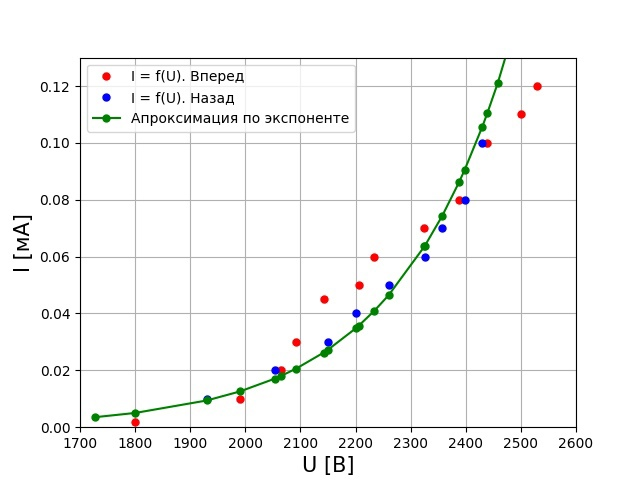
\includegraphics[scale=0.55]{pic2.jpg}
	\caption{ВАХ катода}
	\label{pic2}
\end{figure}

Построим тот же график в координатах Фаулера-Нордгейма:

\begin{figure}[H]
	\centering
	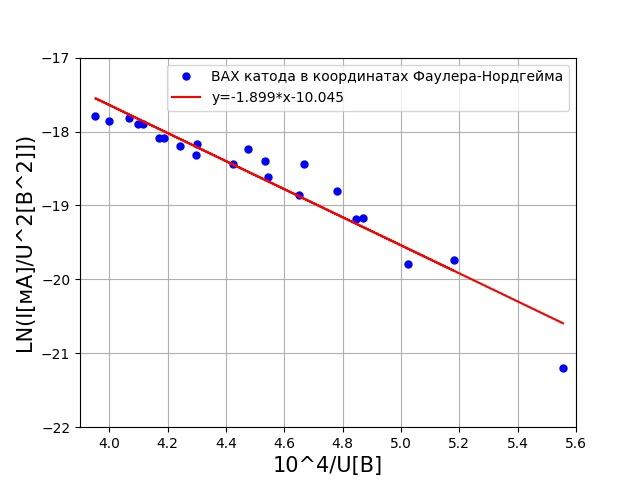
\includegraphics[scale=0.55]{pic3.jpg}
	\caption{ВАХ катода в координатах Фаулера-Нордгейма}
	\label{pic2}
\end{figure}


Из коэффициента наклона $k$ получившейся прямой можем по формуле (1) вычислить форм-фактор $\beta$ (взяв работу выхода углеродных нанотрубок как $\varphi = 4,5$ эВ):

\begin{equation}
    \beta = -0,683\cdot\frac{\varphi^{3/2}}{k}\approx 3,43\cdot 10^{-4} \text{ м}^{-1}.
\end{equation}

Снимем ВАХ лампы с помощью осциллографа. Для этого на один канал мы подаем сигнал с напряжением, подаваемым на катод(рис.\ref{voltage}), на другой - сигнал с напряжением, пропорциональным току, снимаемому с анода (рис.\ref{current}). Зависимость напряжения с анода от напряжения на катод - ВАХ лампы(рис.\ref{BAX})
\begin{figure}[H]
	\centering
	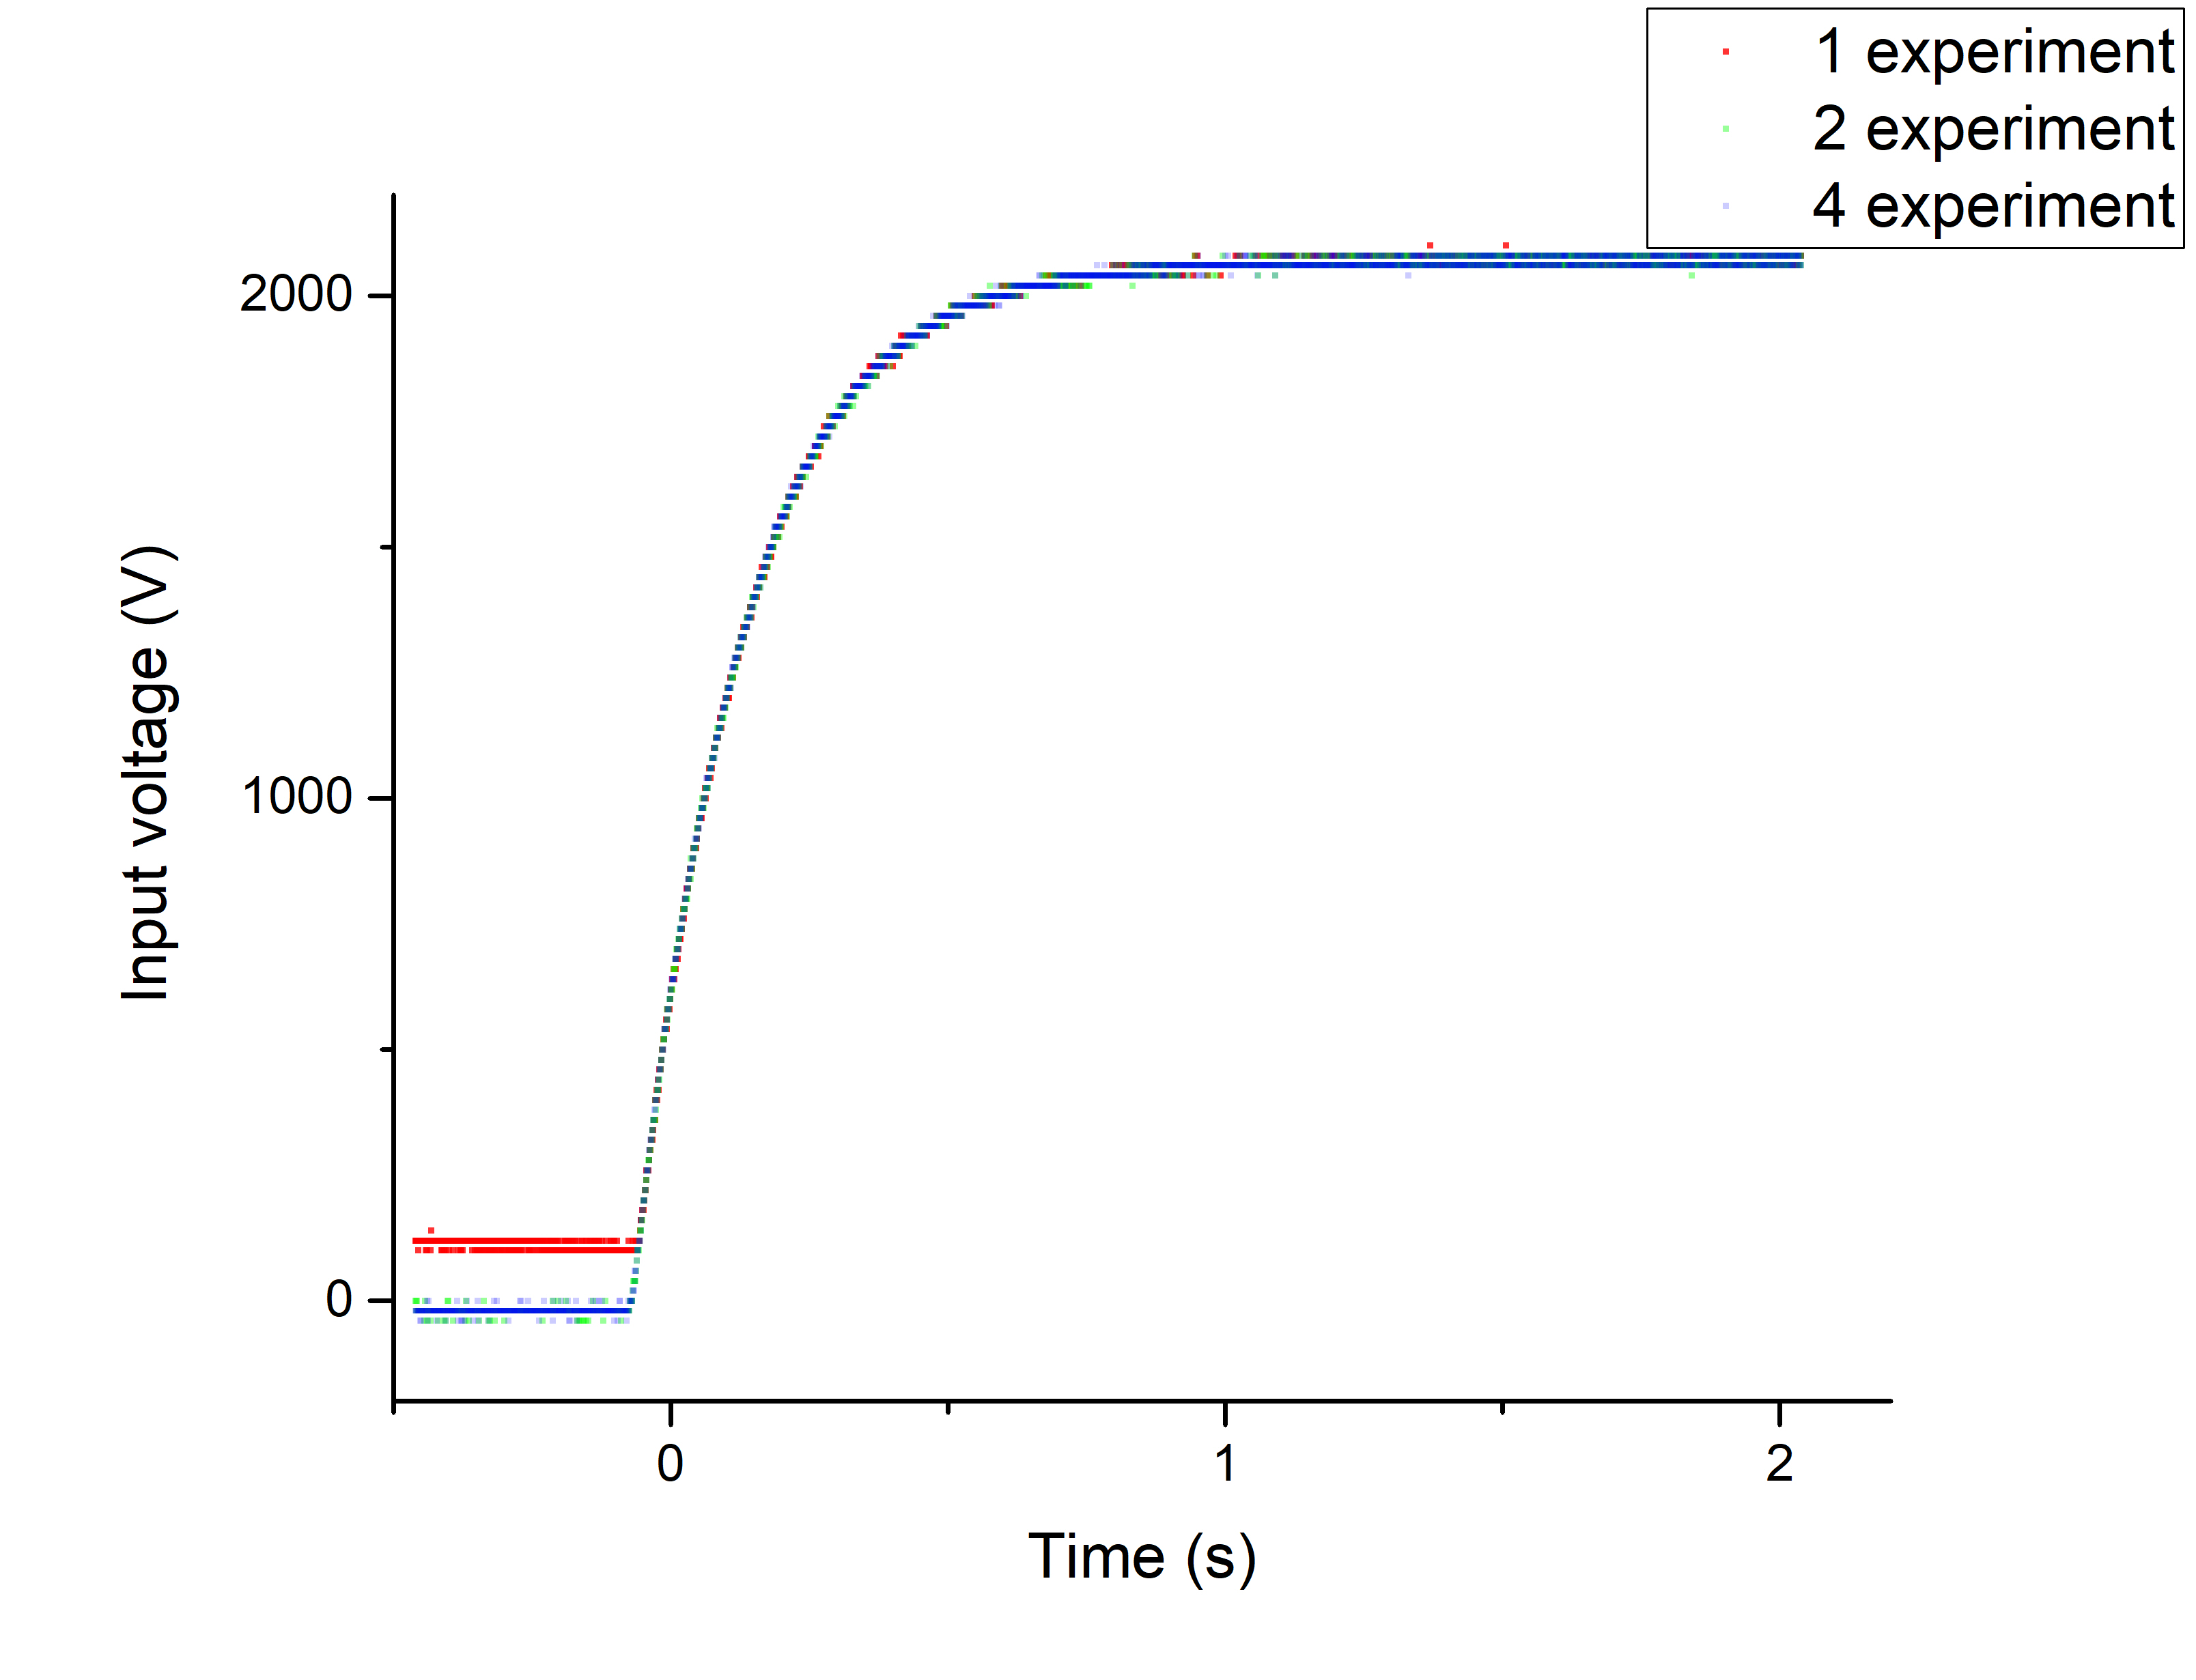
\includegraphics[scale=0.55]{Graph1.jpg}
	\caption{Напряжение, подаваемое на катод}
	\label{voltage}
\end{figure}
\begin{figure}[H]
	\centering
	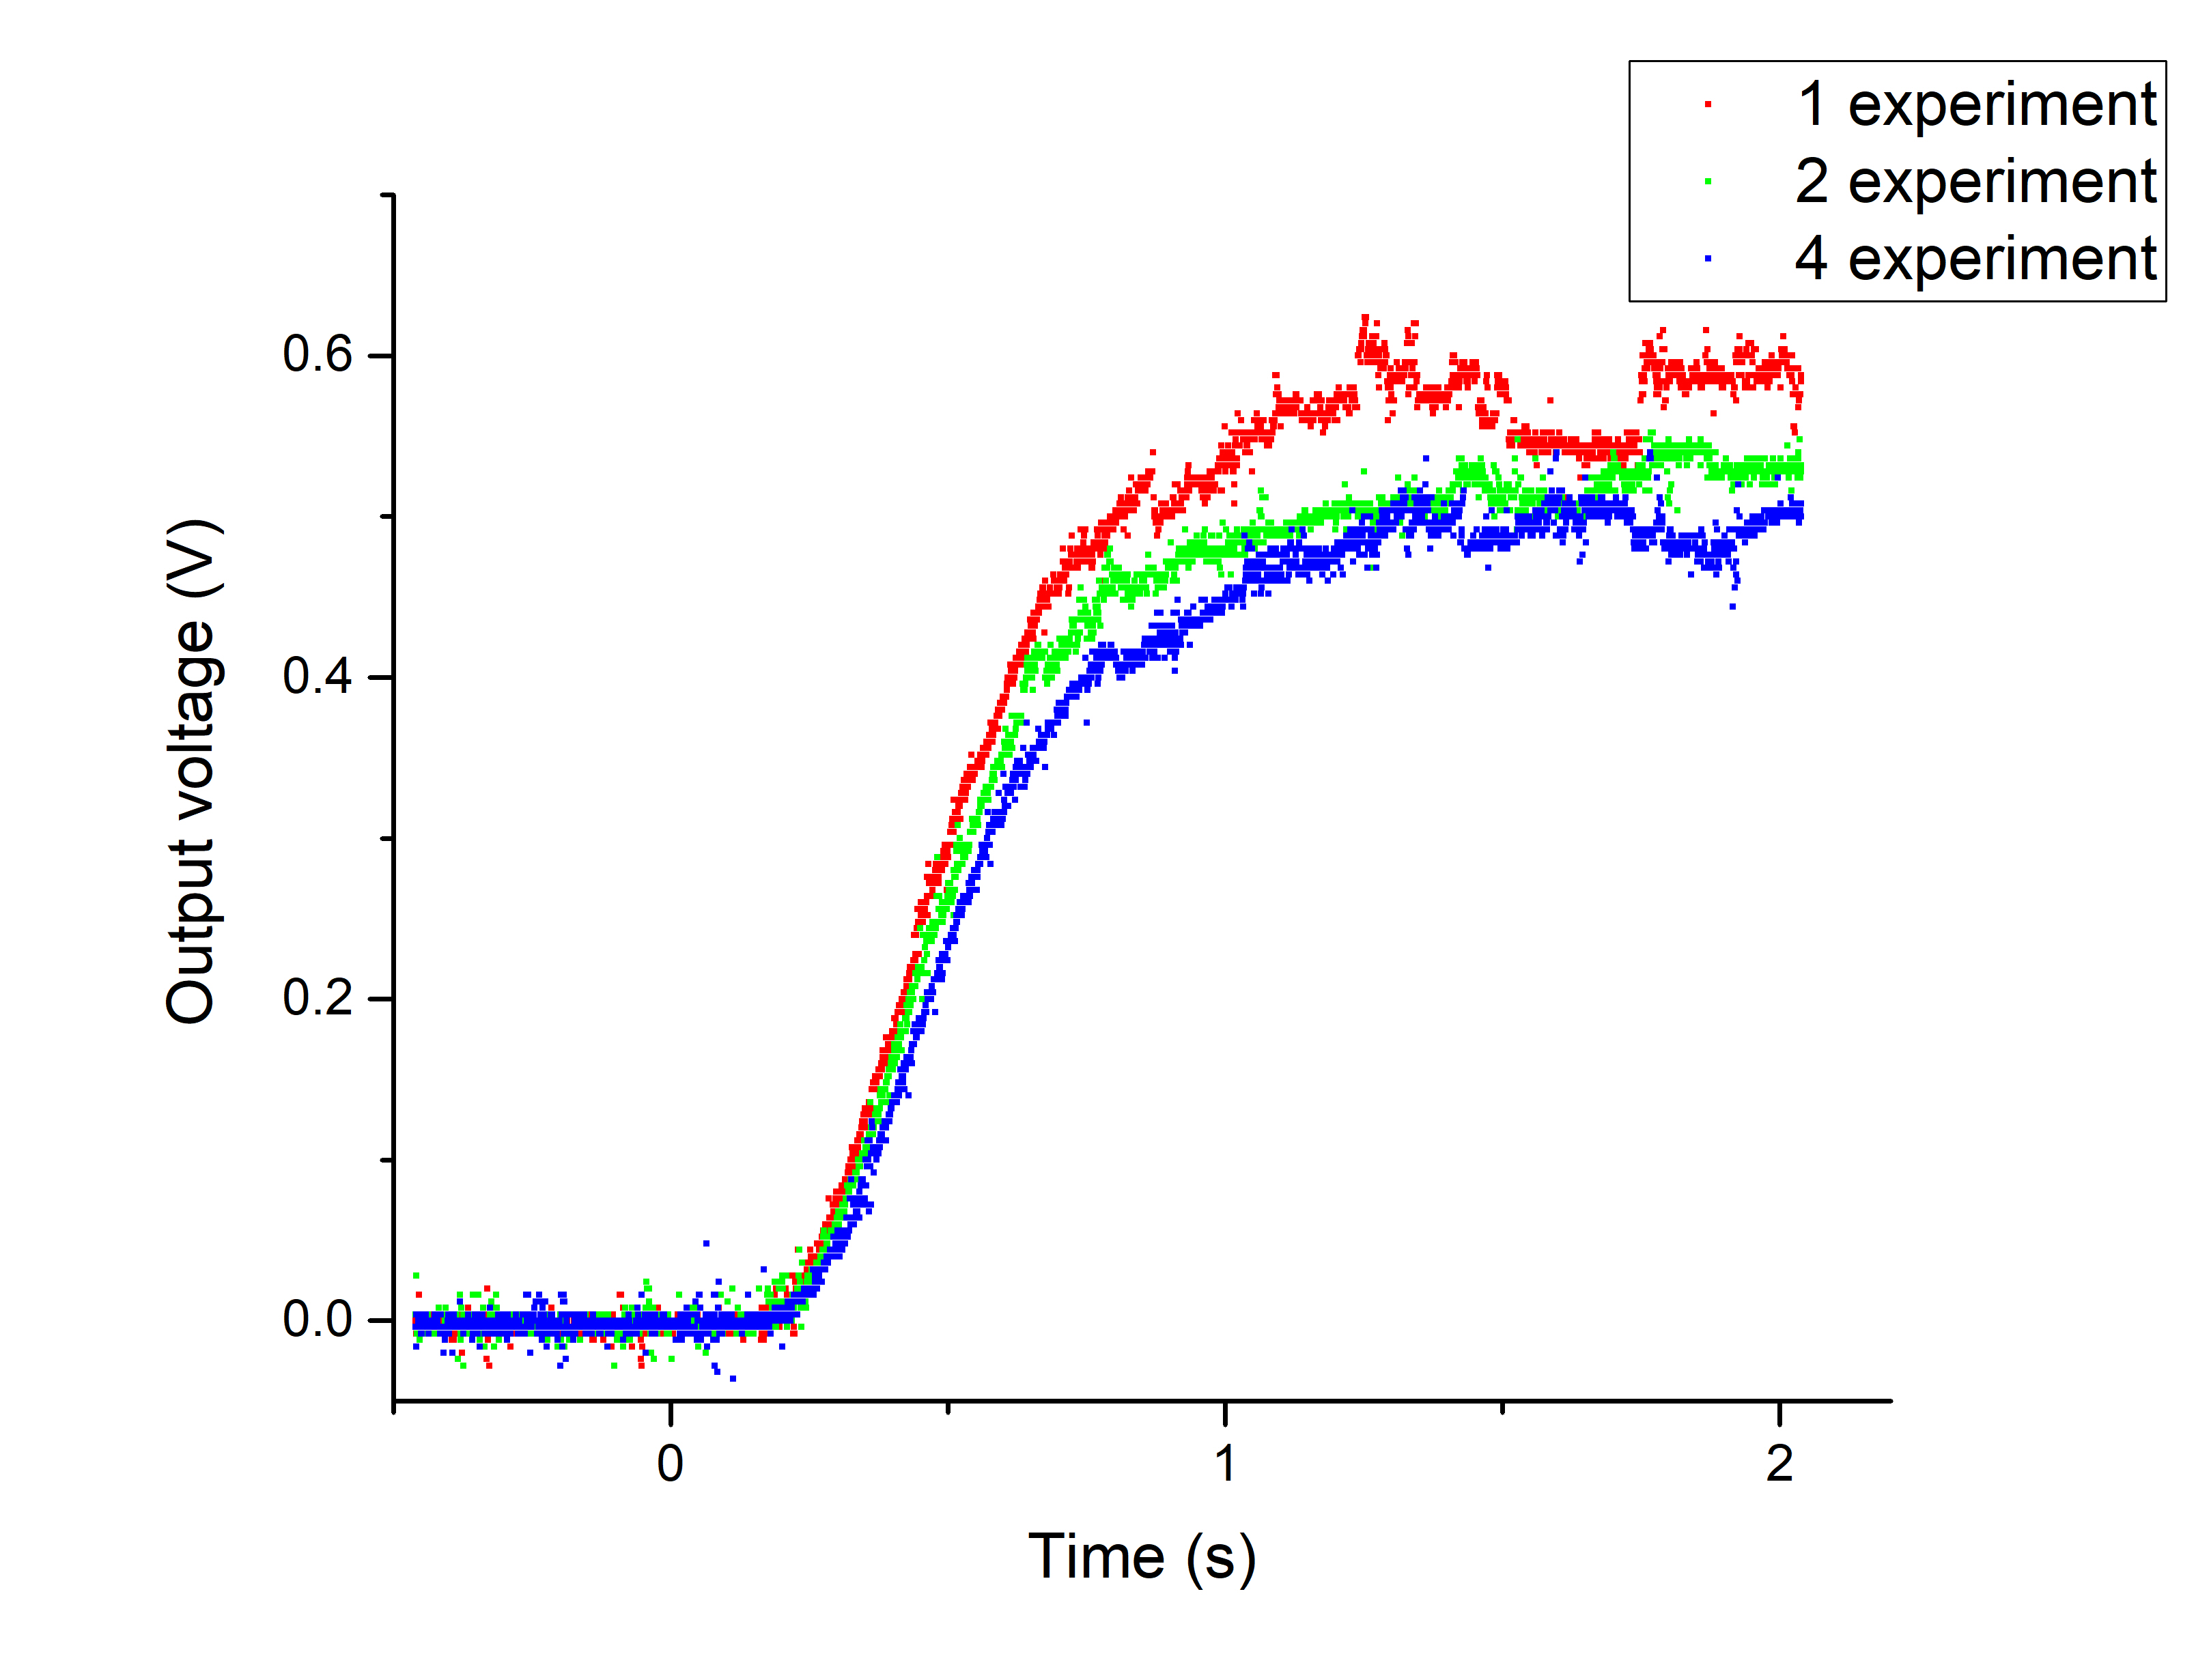
\includegraphics[scale=0.55]{Graph2.jpg}
	\caption{Напряжение, пропорциональное току, снимаемому с анода}
	\label{current}
\end{figure}
\begin{figure}[H]
	\centering
	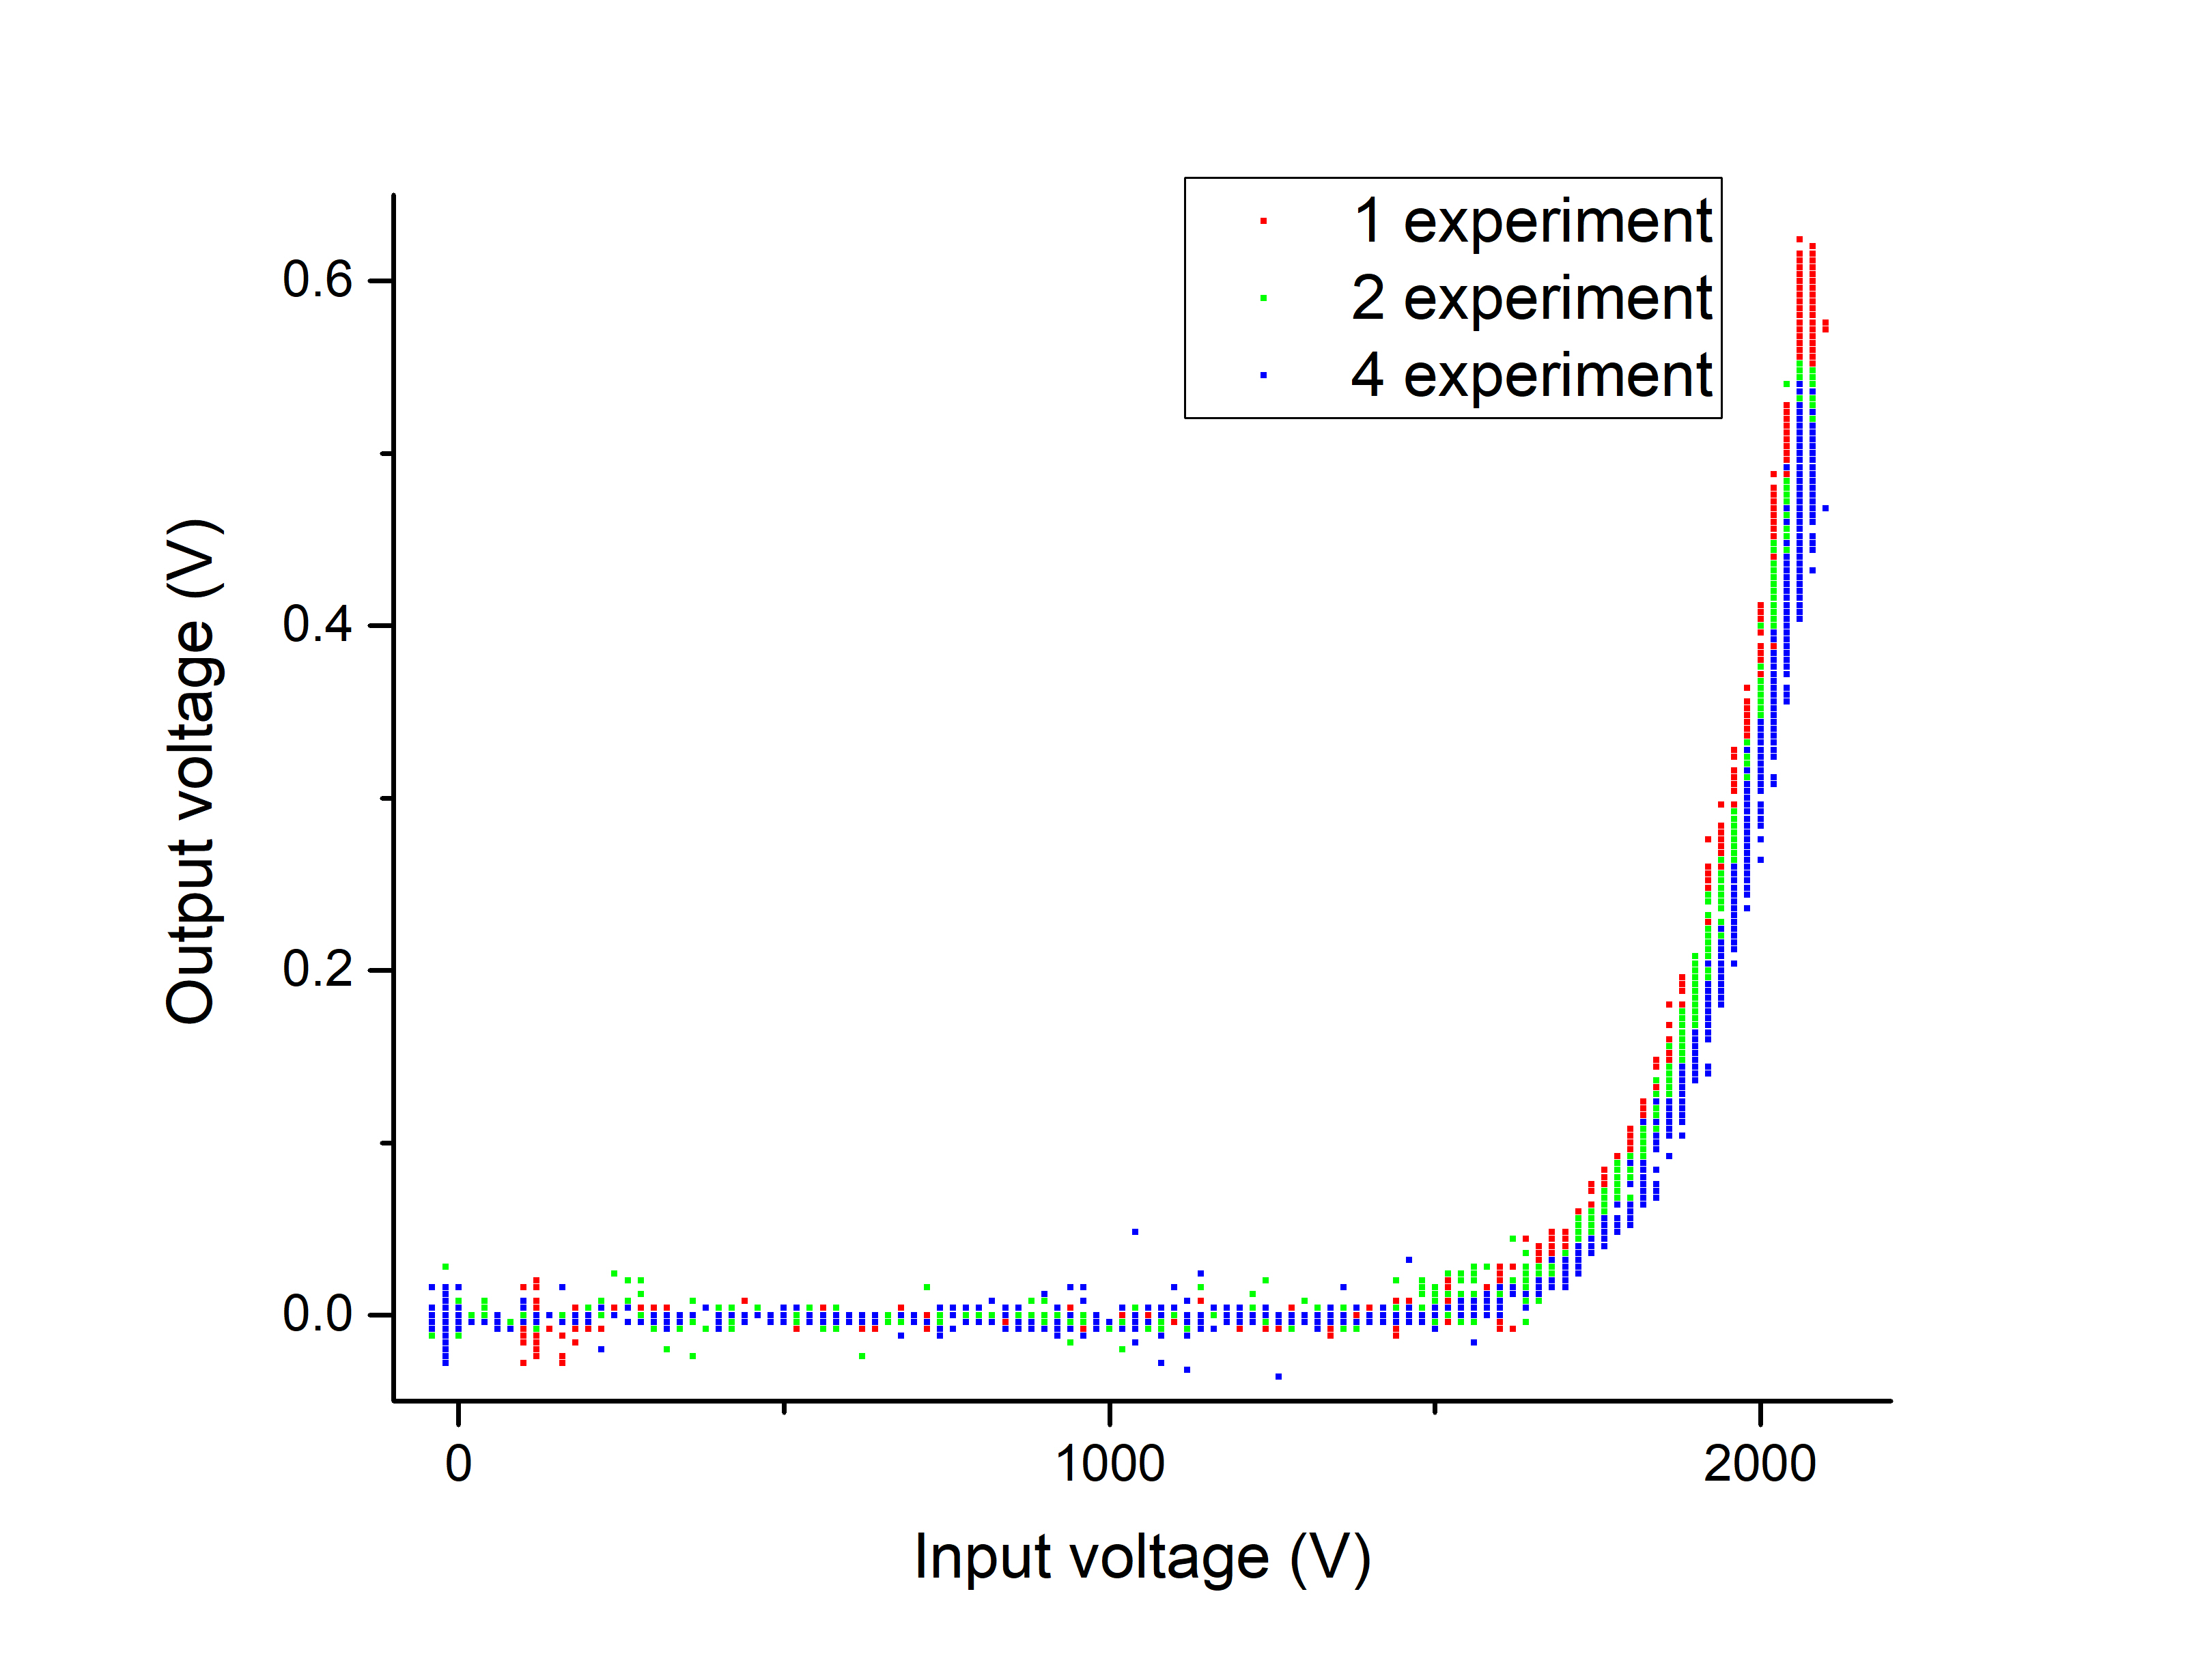
\includegraphics[scale=0.55]{Graph3.jpg}
	\caption{ВАХ лампы}
	\label{BAX}
\end{figure}

\section{Вывод}	
	
В ходе работы мы познакомились с основными автоэмиссионными свойствами угле- родных материалов на примере катода, изготовленного из углеродных волокон; с методом травления пучка углеродных волокон коронным разрядом.
На основании полученных в ходе эксперимента данных нами были проделаны следующие действия:
\begin{enumerate}
    \item Была построена вольт-амперная характеристика катода в координатах $(U;I)$ и координатах Фаулера-Нордгейма $(\frac{1}{U};ln(\frac{I}{U^2}))$
    \item Опираясь на эти графики, мы смогли рассчитать форм-фактор эмиссионного центра:
    \begin{center}
        $\beta\approx 3,43\cdot 10^{-4} \text{ м}^{-1}$
    \end{center}
    \item С помощью осциллографа была получена ВАХ лампы
\end{enumerate}


\end{document}
